
%(BEGIN_QUESTION)
% Copyright 2012, Tony R. Kuphaldt, released under the Creative Commons Attribution License (v 1.0)
% This means you may do almost anything with this work of mine, so long as you give me proper credit

The Fluke corporation sells a software product called {\it DPCTrack2} that may be downloaded and run for a free trial basis.  Locate this software on the Fluke website ({\tt http://www.fluke.com}) and download it to your PC so that you may experiment with it in class.

DPCTrack2 is used to upload calibration specifications to a process calibrator (e.g. the Fluke model 754) prior to instrument technicians performing a field or a bench calibration.  After the calibration(s) have been completed, the calibrator is re-connected to the personal computer so the As-Found and As-Left calibration results may be downloaded to DPCTrack2 for archival.  Thus, DPCTrack2 is useful for calibration {\it workload} management: ensuring all technicians have the information necessary to properly complete mission-critical field instrument calibrations, and ensuring all the calibration data gets properly archived.

\vskip 10pt

In this exercise, you will enter data for a few instruments as they appear on the following P\&ID.  Choose any instruments you wish from the P\&ID (choosing a few within the same control loop would be best, because that would allow you to define a ``Loop'' in the DPCTrack software as well as the instruments themselves), giving yourself license to invent realistic calibration ranges for each of them:

$$\includegraphics[width=15.5cm]{i0007rx01.eps}$$

\vskip 10pt

\filbreak

Your assignment -- at minimum -- is to enter multiple instruments into the DPCTrack2 database, complete with one or more ``Test Point Groups'' specifying calibration parameters for those instruments.  An example of this is shown here:

$$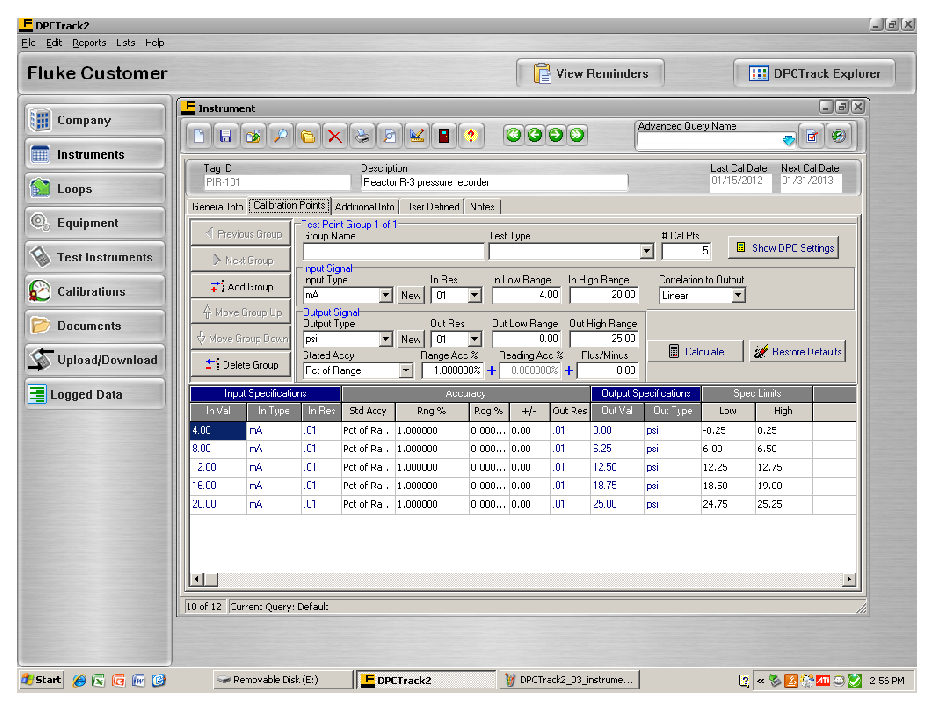
\includegraphics[width=15.5cm]{i02034x01.eps}$$

Beyond that, feel free to experiment with entering more data into the DPCTrack2 database:

\begin{itemize}
\item{} Equipment data (assigning individual instruments to a piece of equipment)
\item{} Loop data (assigning individual instruments to a loop)
\item{} Location data (assigning equipment to certain buildings or other physical locations)
\item{} Technician information
\item{} User's manuals or other instructional documents linked to loops or instruments
\end{itemize}

\underbar{file i02034}
%(END_QUESTION)





%(BEGIN_ANSWER)


%(END_ANSWER)





%(BEGIN_NOTES)

\noindent
{\bf Summary Quiz:}

A demonstration of the configured DPCTrack2 database (multiple instruments entered, complete with calibration point specifications) is sufficient for the summary quiz.

%INDEX% Calibration: Documenting Process Calibrator (Fluke 744/754)
%INDEX% Process: sour water stripping tower (realistic P&ID shown)
%INDEX% Reading assignment: Fluke DPCTrack2 calibration software

%(END_NOTES)


